\documentclass[12pt]{article}
%Gummi|065|=)
\title{\textbf{ Git and \LaTeX{}}}
\author{Kashapov Niyaz}
\date{}
\usepackage[pdftex]{graphicx}
\usepackage{hyperref}
\usepackage[left=2cm,right=2cm,top=2cm,bottom=3cm,bindingoffset=0cm]{geometry}
\usepackage{xcolor}
\usepackage[english]{babel}
\usepackage{cite}
\usepackage{lipsum}  

\makeatletter
\renewcommand{\@listI}{%
\topsep=0pt }
\makeatother
\hypersetup{colorlinks,linkcolor={blue},citecolor={blue},urlcolor={navi}}  
\makeatletter
\let\old@itemize=\itemize
\def\itemize{\old@itemize
\setlength{\itemsep}{0pt}
\setlength{\parskip}{0pt}
\setlength{\leftskip}{0pt}
}
\makeatother
\makeatletter
\let\old@enumerate=\enumerate
\def\enumerate{\old@enumerate
\setlength{\itemsep}{0pt}
\setlength{\parskip}{0pt}
\setlength{\leftskip}{0pt}
}\makeatother

\graphicspath{{noiseimages/}}
\definecolor{linkcolor}{HTML}{0000F0} % цвет ссылок
\definecolor{urlcolor}{HTML}{0459B0} % цвет гиперссылок


\hypersetup{pdfstartview=FitH,linkcolor=linkcolor,urlcolor=urlcolor,colorlinks=true}

\usepackage{graphicx}
\begin{document}

\maketitle

\tableofcontents

\section{Introduction}
\par New file! Test.
\par \LaTeX{}  

\section{Main Part}

%----------------------------------------------------------------------------------------------------------------------------
\subsection{Some words about the Git}
\label{seg:part1}
%----------------------------------------------------------------------------------------------------------------------------
\par Git is an open source distributed version control system (DVCS), mainly used for source code management (SCM), with an emphasis on speed. Git was initially designed and created by Linus Torvalds for Linux kernel development. Git operates on a decentralized architecture, so every Git working directory is a full-fledged repository with a complete history and full revision-tracking capabilities, and is not dependent upon network access or a central server.

\par Unlike popular non-distributed predecessors, such as Subversion and CVS, Git only needs a central server for one thing: publishing changes to users of that server. You can equally share changes directly with other people without the need to consult a central hub.

\par Also unlike the monolithic design of Subversion and CVS, Git follows the typical Unix philosophy with a great many small components that do single atomic tasks. Of course, only a few of the dozens of separate commands are often used. Most commands are for specialized actions, and a good portion are designed to be called by shell scripts rather than users.
\cite{gitbook}

%----------------------------------------------------------------------------------------------------------------------------
\subsection{Services of GitHub}
\par GitHub is a web-based Git or version control repository and Internet hosting service. It is mostly used for code. It offers all of the distributed version control and source code management (SCM) functionality of Git as well as adding its own features. It provides access control and several collaboration features such as bug tracking, feature requests, task management, and wikis for every project.

\par GitHub offers both plans for private and free repositories on the same account which are commonly used to host open-source software projects. As of April 2017, GitHub reports having almost 20 million users and 57 million repositories, making it the largest host of source code in the world.

\par GitHub has a mascot called Octocat, a cat with five tentacles and a human-like face
\subsubsection{Features}
In addition to source code, GitHub supports the following formats and features:
\begin{itemize}
\item Documentation, including automatically rendered README files in a variety of Markdown-like file formats (see README files on GitHub)
\item Issue tracking (including feature requests) with labels, milestones, assignees and a search engine
\item Wikis
\item Pull requests with code review and comments
\item Commits history
\item Graphs: pulse, contributors, commits, code frequency, punch card, network, members
\item Integrations Directory
\item Unified and split diffs
\item Email notifications
\item Option to subscribe someone to notifications by @ mentioning them.
\item Emojis[16]
\item GitHub Pages: small websites can be hosted from public repositories on GitHub. The URL format is http://username.github.io.
\item Nested task-lists within files
\item Visualization of geospatial data
\item 3D render files that can be previewed using a new integrated STL file viewer that displays the files on a "3D canvas". \item The viewer is powered by WebGL and Three.js.
\item Photoshop's native PSD format can be previewed and compared to previous versions of the same file.
\item PDF document viewer
\end{itemize}

\subsubsection{Required software}
\par Necessary libraries:
\begin{itemize}
	\item curl-devel 
	\item expat-devel 
	\item gettext-devel 
	\item openssl-devel
	\item zlib-devel
\end{itemize}
\subsubsection{Git in use}
\par How to use:
\begin{enumerate}
\item Download and install \texttt{git} to the OS
%_________
		\begin{description}
			\item{\textbf{Ubuntu}} \texttt{ \# yum install git-core }
			\item{\textbf{Fedora}}  \texttt{ \# apt-get install git }
		\end{description}
%_________
\item Configure \texttt{git}
\begin{verbatim}
$ git config --global user.name "User Looser"
$ git config --global user.email u.looser@example.com
$ git config --global core.editor nano
\end{verbatim}
\item Go to the project directory
\item Use \texttt{\$ git init} commnad to initialize and make .git repository
\end{enumerate}


\begin{figure}[!h]
\centering
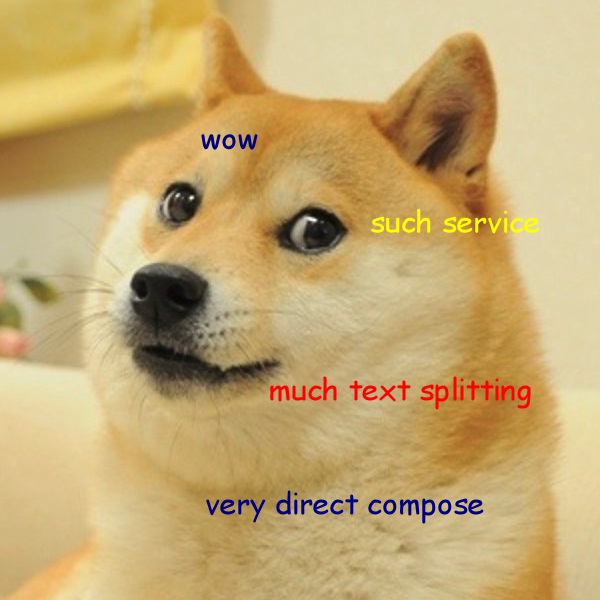
\includegraphics[scale=0.50]{doge.png}
\caption{Picture from directory}
\label{dogepic}
\end{figure}
%----------------------------------------------------------------------------------------------------------------------------

\subsection{Part 2}
%----------------------------------------------------------------------------------------------------------------------------


%----------------------------------------------------------------------------------------------------------------------------


\subsection{Part 3}
%----------------------------------------------------------------------------------------------------------------------------


%----------------------------------------------------------------------------------------------------------------------------





\section{Results}

\section{Appendices}

\newpage

\begin{thebibliography}{9} 
\bibitem{gitbook} Git, WikiBooks \url{https://en.wikibooks.org/wiki/Git}
\bibitem{github} GitHub, Wikipedia \url{https://en.wikipedia.org/wiki/GitHub}
\end{thebibliography} 

\end{document}